% Figure M8 hero prototype : generated by experiments/m8_finance.py --hero.
% Preview-only; not yet linked from the main manuscript.
\begin{figure}[t]
 \centering
 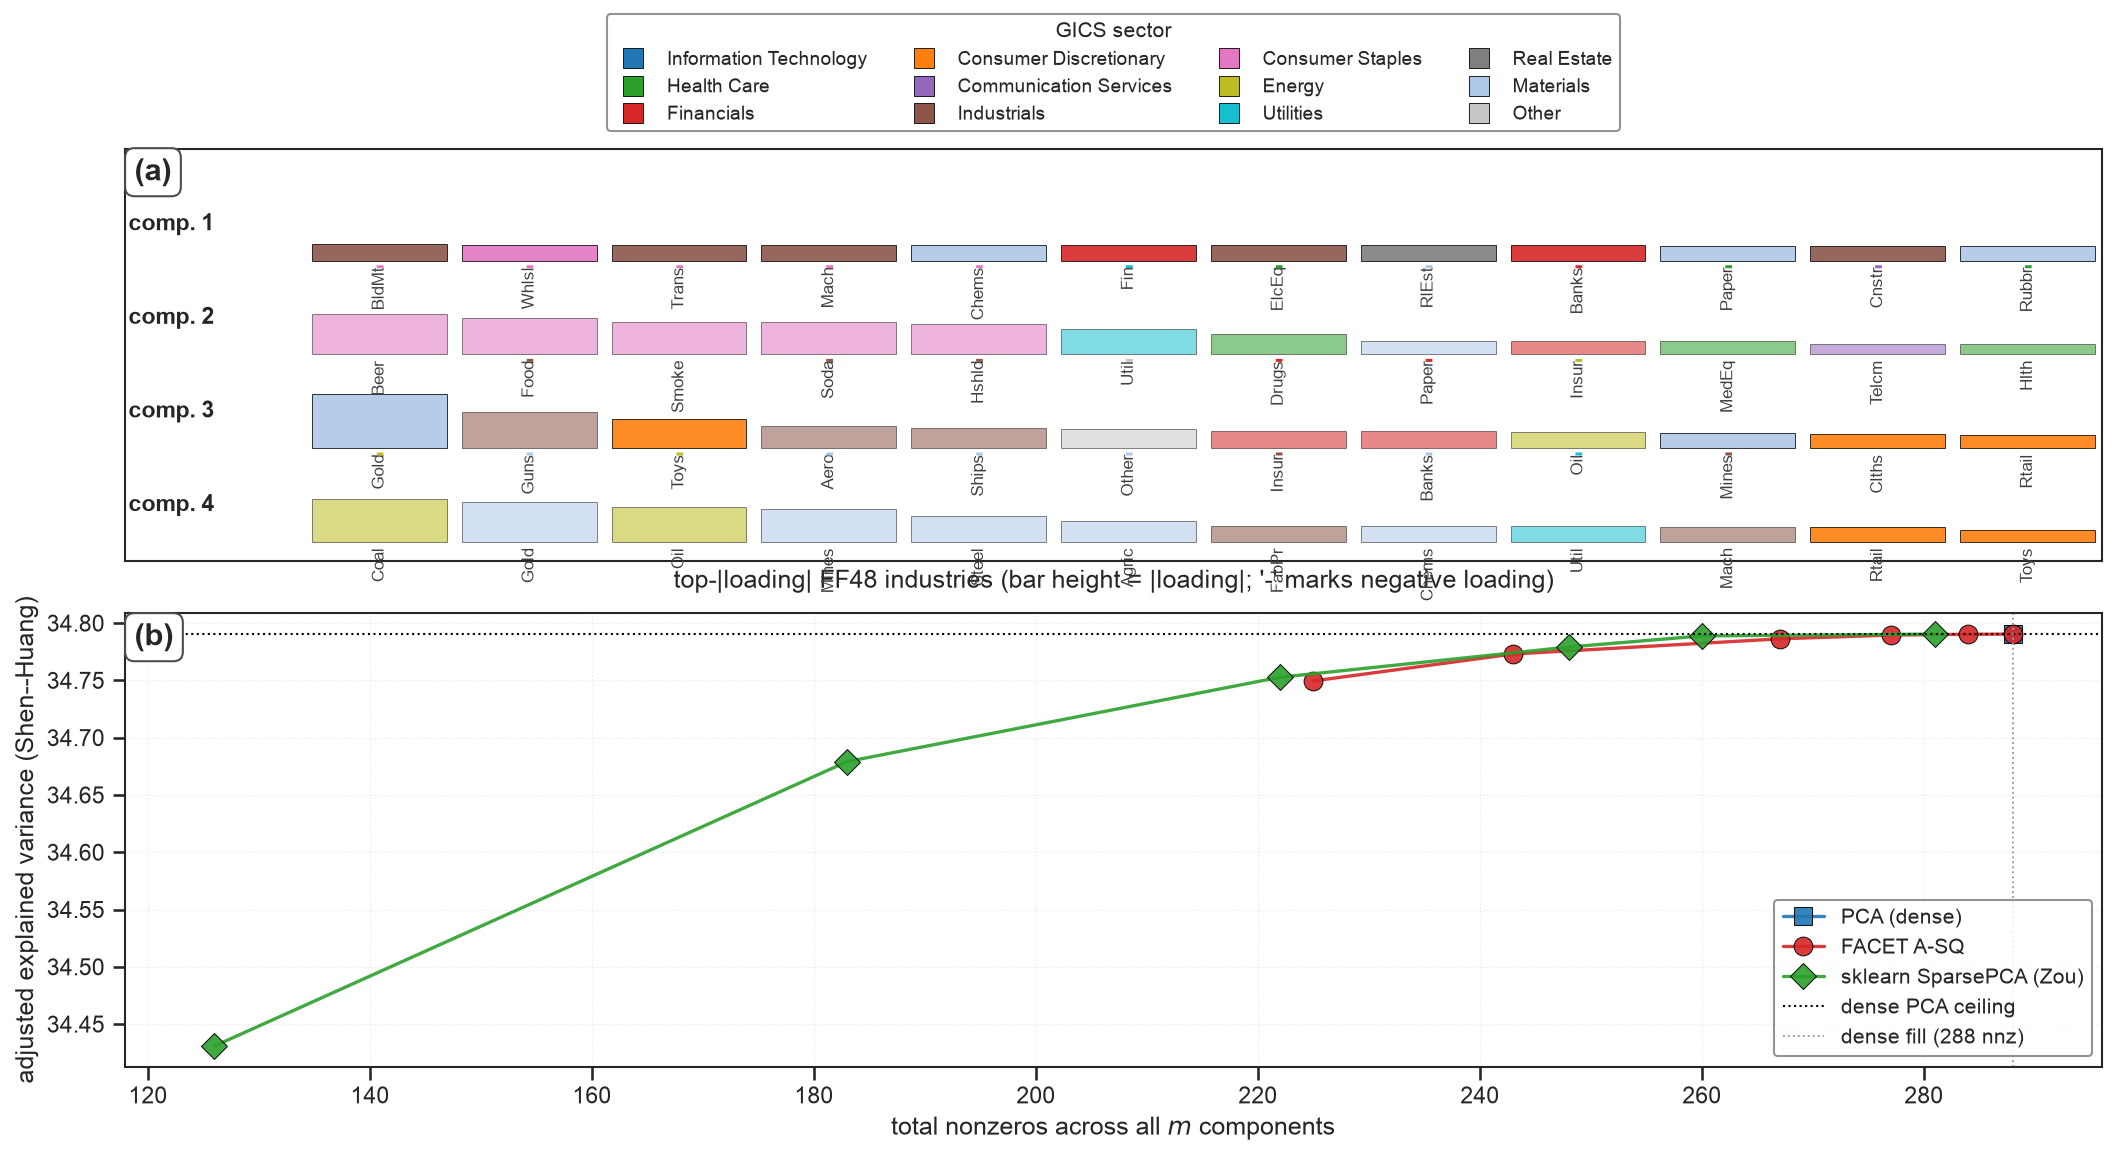
\includegraphics[width=\linewidth]{../shared/figures/generated/m8_finance_hero.png}
 \caption{\textbf{M8: sparse risk factors on Fama-French 48 industry daily returns.} 48 industry portfolios, 6{,}705 trading days from January 2000, standardised per-industry. \textbf{(a)}~Top-four FACET A-SQ components at $\gamma{=}0.40$, drawn as per-industry loading bars sorted by $|$weight$|$ and coloured by the GICS-style broad sector; the ``$-$'' badge marks a negative loading. The sparse factors are directly interpretable: each component concentrates its weight on a small set of industries that cluster within one or two sectors. \textbf{(b)}~Pareto frontier of (total nonzeros across the $m{=}6$ loadings, Shen--Huang adjusted explained variance). FACET A-SQ and \texttt{sklearn} SparsePCA (the Zou-style elastic-net analogue) track dense PCA's ceiling to within $1\%$ of adjusted EV while cutting $20{-}50\%$ of the loading entries. Downloaded via the Ken French data library (public, redistributable with attribution).}
 \label{fig:m8-finance-hero}
\end{figure}
